\begin{frame}
\frametitle{Métodos e Procedimentos}
\framesubtitle{Visão geral}

\begin{figure}[hbt]
	\begin{center}
		\caption{Diagrama de bloco das etapas de desenvolvimento}
		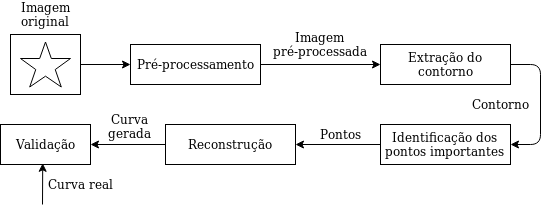
\includegraphics[width=1\textwidth]{img/diagrama.png}
	\end{center}
\end{figure}

\end{frame}

% pre processamento
\subsection{Pré-processamento}

\begin{frame}
\frametitle{Pré-processamento}

\destaq{Objetivos:}
\begin{itemize}
\item Suavizar a imagem;
\item Remover ruídos.
\end{itemize}

\bigskip
\destaq{Técnicas utilizadas:}
\begin{itemize}
	\item Filtro gaussiano ou Perona-Malik;
	\item Binarização por Otsu;
	\item Operadores morfológicos (erosão e dilatação).
\end{itemize}
\end{frame}

\begin{frame}
\frametitle{Pré-processamento}

\destaq{Extração do contorno:}
\begin{itemize}
	\item Acompanha a borda do objeto, e verifica se seus vizinhos também pertencem ao objeto.
\end{itemize}

\begin{figure}[hbt]
	\begin{center}
		\caption{Método \textit{contour following}~\cite{book_shape}}
		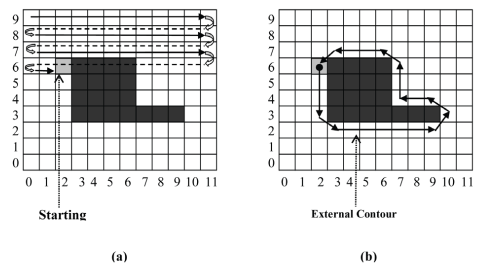
\includegraphics[width=0.6\textwidth]{img/contorno.png}
	\end{center}
\end{figure}
\end{frame}

% calculo da curvatura + contorno
\subsection{Curvatura}

\begin{frame}
\frametitle{Escolha dos pontos}

\begin{itemize}
\item \destaq{Pontos linearmente espaçados:} índices igualmente espaçados entre si;
\medskip
\item \destaq{Escolha de pontos pela curvatura:} pontos com maior valor absoluto de curvatura.
\end{itemize}

\end{frame}

\begin{frame}
\frametitle{Curvatura}
\framesubtitle{Curvatura contínua}

Seja uma curva regular parametrizada por $t \rightarrow (x(t), y(t))$, em que $x(t)$ e $y(t)$ são funções de classe $C^2$. Sua curvatura é dada por:
$$\kappa (t) = \frac{x'(t) y''(t) - y'(t) x''(t)}{(x'(t)^2 + y'(t)^2)^{3/2}}$$   

\end{frame}


\begin{frame}
\frametitle{Curvatura discreta}
	
	No caso discreto, precisa-se calcular a derivada discreta.
	
	\medskip
	
	Utilização de \textbf{métodos espectrais de Fourier} \cite{brethwashington} e \textbf{filtro gaussiano} para suavizar e reduzir erros.
	
\end{frame}

\begin{frame}
\frametitle{Curvatura discreta}

Seja $u_j$ uma aproximação discreta da função $u(x)$, com $n$ pontos de amostra $x_j \in h, 2h, \dots, ih, \dots, 2\pi - h, 2\pi$, onde $h = 2\pi/n$. Pode-se aplicar a transformada rápida de Fourier (FFT) em $u_j$, tal que $FFT(u_j) \equiv \hat{u}_k$, em que $k \in \frac{-n}{2}+1, \dots, \frac{n}{2}$. Sabe-se que:

\medskip

$$FFT \left (\frac{\partial u_j}{\partial x} \right) \equiv i k \hat{u}_k$$

\medskip

Assim, para obter o valor da derivada, basta calcular a transformada rápida inversa IFFT.
\end{frame}


% reconstrucao - sorkine
\subsection{Reconstrução}

\begin{frame}
\frametitle{Reconstrução}
\framesubtitle{Definições}

\destaq{Modelagem geométrica:} conjunto de técnicas e algoritmos utilizados para modelar determinadas formas matemáticas, sujeitas a condições particulares de forma e suavidade.


\medskip
Uma forma possível de se modelar é com a utilização do \destaq{operador discreto de Laplace-Beltrami} \cite{Sorkine2006}.

\end{frame}

\begin{frame}
\frametitle{Coordenadas diferenciais}

Seja uma malha triangular $\mathcal{M} = (V, E, F)$. Cada vértice $\mathbf{v}_i \in V$ possui uma representação cartesiana dada por $\mathbf{v}_i = (x_i,y_i,z_i)$.

\medskip

\destaq{Coordenadas diferenciais} (ou $\mathbf{\delta}$\textit{-coordenadas}) de $\mathbf{v}_i$ são definidas como a diferença entre a coordenada cartesiana e o centro de massa de seus vizinhos imediatos na malha:

\begin{equation}
	\mathbf{\delta}_i = (\mathbf{\delta}_i^{(x)}, \mathbf{\delta}_i^{(y)}, \mathbf{\delta}_i^{(z)}) = \mathbf{v}_i - \frac{1}{d_i} \sum_{j \in N(i)} \mathbf{v}_j,
	\label{eq_delta}
\end{equation}

\noindent em que $N(i) = \{j|(i,j) \in E$\} e $d_i = |N(i)|$.

\end{frame}

\begin{frame}
\frametitle{Coordenadas diferenciais}
\framesubtitle{Transformação para $\delta$-coordenadas}

Seja $A$ a matriz de adjacências da malha:

$$
A_{ij} = \begin{cases}
	1&(i, j) \in E\\
	0&\text{caso contrário.}
\end{cases}
$$

e $D$ a matriz diagonal tal que

$$D_{ii} = d_{i} = |N(i)| = \text{número de vértices adjacentes a }i$$

A matriz $L$ de transformação de coordenadas cartesianas para as coordenadas diferenciais é:

\begin{equation}
	L = I - D^{-1}A.
\end{equation}

\end{frame}

\begin{frame}
\frametitle{Coordenadas diferenciais}
\framesubtitle{Transformação para $\delta$-coordenadas}

É mais comum utilizar a versão simétrica de $L$, $L_s$, tal que:

$$L_s = DL = D - A$$

e cada célula pode ser calculada por:

\begin{equation}
	(L_s)_{ij} = \begin{cases}
		d_i&i=j\\
		-1&(i, j) \in E\\
		0&\text{caso contrário.}
	\end{cases}
\end{equation}


\end{frame}

\begin{frame}
\frametitle{Coordenadas diferenciais}
\framesubtitle{Transformação para $\delta$-coordenadas}

Temos:

$$L_s \textbf{x} = \delta^{(x)}$$
$$L_s \textbf{y} = \delta^{(y)}$$
$$L_s \textbf{z} = \delta^{(z)}$$

e $L_s$ é denominado \destaq{Laplaciano topológico} da malha $\mathcal M$.

\end{frame}

\begin{frame}
\frametitle{Coordenadas diferenciais}
\framesubtitle{Discretização de Laplace-Beltrami}

Se considerar $\mathcal{M}$ uma aproximação linear por partes de uma superfície suave,

$$\delta_i = \frac{1}{d_i} \sum_{j \in N(i)}(\mathbf{v_i} - \mathbf{v_j})$$

é uma discretização de

$$\frac{1}{|\gamma|} \int_{v \in \gamma} (v_i - v) dl(v)$$

em que $\gamma$ é uma curva de uma superfície fechada simples em volta de $v_i$ e $|\gamma|$ é o comprimento de $\gamma$.

\end{frame}

\begin{frame}
\frametitle{Coordenadas diferenciais}
\framesubtitle{Discretização de Laplace-Beltrami}

Sabe-se que:

$$\lim\limits_{|\gamma|\rightarrow 0} \frac{1}{|\gamma|} \int_{v \in \gamma} (v_i - v) dl(v) = - H(v_i) n_i$$

em que $H(v_i)$ é a curvatura média de $v_i$ e $n_i$ é a normal à superfície.

\medskip

\begin{itemize}
	\item Intuitivamente, as $\delta$-coordenadas \destaq{encapsulam a forma local da superfície}:
	\begin{itemize}
		\item A direção aproxima o vetor normal;
		\item A norma aproxima a curvatura média;
	\end{itemize}
\end{itemize}

\end{frame}

\begin{frame}
\frametitle{Aplicações}
\framesubtitle{Representação eficiente de formas}

Com apenas informações de conectividade da malha e alguns pontos fixados (denominados vértices âncora), é possível aproximar toda a geometria, a partir da resolução do sistema pelo \destaq{método dos mínimos quadrados}:

\begin{equation}\label{eq:sisrecover}
	\left( \frac{L}{I_{m \times m} | 0} \right) \mathbf{x'} = \begin{pmatrix}
		0\\
		c_{1:m}^{(x)}
	\end{pmatrix}
\end{equation}

em que $c = \{v_1, v_2, \dots, v_m\}$ são os pontos âncora escolhidos como amostra.

\end{frame}